% Metódy inžinierskej práce

\documentclass[10pt,twoside,slovak,a4paper]{article}

\usepackage[slovak]{babel}
%\usepackage[T1]{fontenc}
\usepackage[IL2]{fontenc} % lepšia sadzba písmena Ľ než v T1
\usepackage[utf8]{inputenc}
\usepackage{graphicx}
\usepackage{url}
\usepackage{hyperref}

\usepackage{cite}

\pagestyle{headings}

\title{Detekcia falošných online recenzií na základe jazykových a behaviorálnych príznakov\thanks{Semestrálny projekt v predmete Metódy inžinierskej práce, ak. rok 2026/27, vedenie: Meno Priezvisko}}

\author{Matvii Nosenko, Volodymyr Nedoluha, Danylo Nikolenko\\[2pt]
	{\small Slovenská technická univerzita v Bratislave}\\
	{\small Fakulta informatiky a informačných technológií}\\
	{\small \texttt{xnosenko@stuba.sk, xnedoluha@stuba.sk, xnikolenkod@stuba.sk}}
	}

\date{\small 29. september 2026}



\begin{document}

\maketitle

\begin{abstract}
Online recenzie výrazne ovplyvňujú rozhodovanie spotrebiteľov, no ich dôveryhodnosť narúšajú falošné recenzie generované firmami, platenými recenzentmi či automatizovanými nástrojmi. Tento článok prináša prehľad súčasných metód detekcie falošných recenzií so zameraním na porovnanie jazykových (textových) a behaviorálnych (na správaní recenzenta založených) príznakov.
\end{abstract}


% --- Vrchná štruktúra článku (zatiaľ len nadpisy, obsah doplníme neskôr) ---

\section{Úvod}

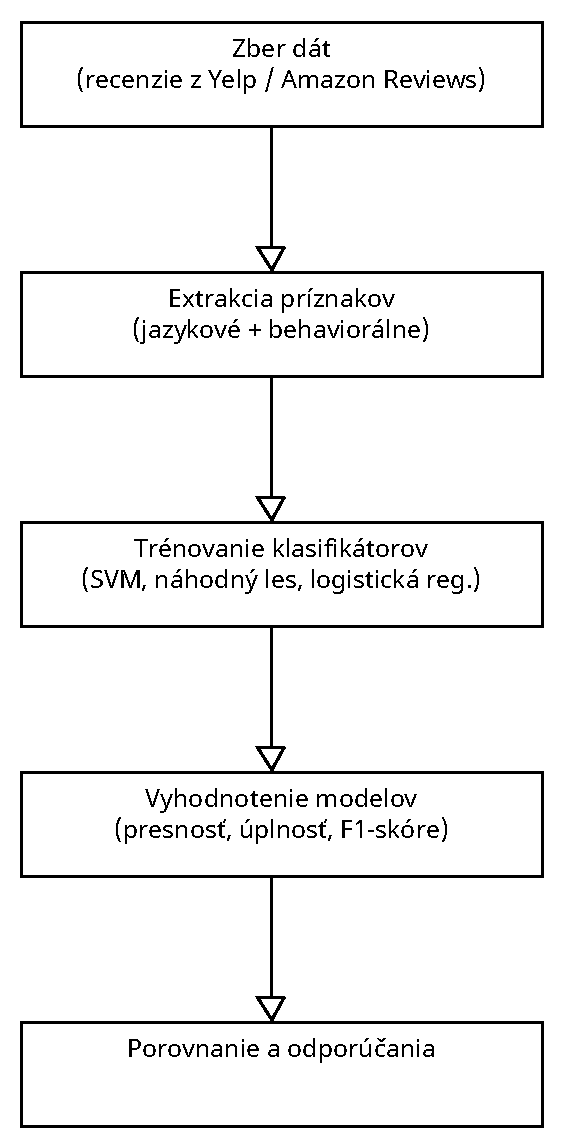
\includegraphics[scale=1.0]{diagram.pdf}

\section{Súvisiace práce} \label{suvisiace}

\section{Jazykové príznaky} \label{jazykove}

\section{Behaviorálne príznaky} \label{behavioralne}

\section{Porovnanie prístupov} \label{porovnanie}

\section{Záver} \label{zaver}


% \bibliography{literatura}
% \bibliographystyle{plain}
\end{document}